\documentclass[conference]{IEEEtran}

\usepackage[T1]{fontenc}
\usepackage[utf8]{inputenc}
\usepackage{cite}
\usepackage{url}
\usepackage{booktabs}
\usepackage{multirow}
\usepackage{array}
\usepackage{tabularx}
\usepackage{graphicx}
\usepackage{xcolor}
\usepackage{amsmath}
\usepackage{tikz}
\usetikzlibrary{arrows.meta,positioning,shapes.geometric,fit,backgrounds}

\definecolor{accentblue}{RGB}{14,165,233}
\definecolor{accentgreen}{RGB}{22,163,74}
\definecolor{accentorange}{RGB}{249,115,22}
\definecolor{accentpurple}{RGB}{147,51,234}
\definecolor{softgray}{RGB}{245,247,250}

\title{A DevSecOps Security Monitoring Architecture for LogiFlow:\\
From Vulnerable Baseline to Continuous Threat Visibility}

\author{\IEEEauthorblockN{Andersson David Sanchez Mendez, Cristian Santiago Pedraza Rodriguez, Jeisson David Sanchez Gomez}
\IEEEauthorblockA{Escuela Colombiana de Ingenieria Julio Garavito\\
SPTI - Seguridad y Privacidad de Tecnologias de la Informacion\\
Bogota, Colombia\\
Email: \{andersson.sanchez, cristian.pedraza-r, jeisson.sanchez\}@escuelaing.edu.co}}

\begin{document}
\maketitle

\begin{abstract}
LogiFlow is a real-time microservices platform for fleet routing where service trust, operational continuity, and data integrity are critical. This paper presents a complete DevSecOps security monitoring architecture that compares an intentionally vulnerable baseline against a hardened production-oriented design. We identify attack surfaces in API, WebSocket, webhook, container runtime, and CI/CD supply-chain paths, and prioritize threats through STRIDE and OWASP Top 10 (2021). The proposed architecture integrates shift-left controls (CodeQL, Semgrep, npm audit, GitLeaks, Trivy, OWASP ZAP) with shift-right telemetry (Falco, Prometheus, Loki, Grafana) and distributed tracing (OpenTelemetry, Tempo). Results from test scenarios TC-01 to TC-10 show effective mitigation of high-priority exploit paths such as unauthorized socket access, unauthenticated webhook injection, and request-flood abuse, while improving forensic readiness and triage speed. The resulting artifact provides a reusable blueprint for academic and industry teams implementing continuous security in distributed systems.
\end{abstract}

\begin{IEEEkeywords}
DevSecOps, Microservices Security, OWASP Top 10, STRIDE, Runtime Monitoring, Falco, Prometheus, Loki, Grafana, OpenTelemetry, Tempo
\end{IEEEkeywords}

\section{Introduction}
Modern logistics platforms are increasingly event-driven and distributed, which improves responsiveness but expands attack surface and detection latency. In LogiFlow, critical routing decisions are produced by interconnected services (gateway, real-time channels, optimization, automation, and persistence), making security failures operationally expensive.

This work addresses the SPTI objective of security-by-design with measurable controls by implementing and validating a full DevSecOps security layer over LogiFlow. The contribution is threefold:
\begin{enumerate}
\item A reproducible baseline-to-hardened architecture comparison with explicit vulnerability-to-control mapping.
\item An integrated CI/CD security pipeline that combines SAST, SCA, secrets detection, container scanning, and DAST.
\item A continuous monitoring and triage stack that correlates metrics, logs, runtime anomalies, and traces for faster incident response.
\end{enumerate}

\section{Background}
\subsection{OWASP Top 10 and STRIDE}
OWASP Top 10 (2021) is used as the vulnerability taxonomy to classify weaknesses in access control, authentication, misconfiguration, outdated dependencies, and monitoring gaps \cite{owasp2021}. STRIDE guides threat modeling across spoofing, tampering, repudiation, information disclosure, denial of service, and elevation of privilege.

\subsection{NIST CSF and SGSI Perspective}
NIST CSF provides a governance structure through Identify, Protect, Detect, Respond, and Recover functions \cite{nistcsf}. This aligns with SGSI-style traceability where each control must map to evidence, validation criteria, and operational ownership.

\subsection{DevSecOps Principles}
The architecture follows shift-left plus shift-right security: prevent defects early in CI while maintaining runtime anomaly detection and observability in production-like environments \cite{devsecopsnist}.

\section{LogiFlow System Description}
\subsection{Service Topology}
LogiFlow uses a microservices topology with heterogeneous technologies: NestJS gateway, Socket.IO real-time service, VROOM-based optimizer, Redis, PostgreSQL, Python predictor, and n8n automation.

\begin{table}[htbp]
\caption{Core LogiFlow Services and Security-Relevant Role}
\centering
\begin{tabularx}{\linewidth}{>{\raggedright\arraybackslash}p{2.1cm} >{\raggedright\arraybackslash}p{2.0cm} X}
\toprule
Service & Tech Stack & Security-Relevant Role \\
\midrule
Gateway & NestJS, JWT, Prisma & API boundary, token issuance, webhook protection, security metrics \\
Realtime & Node.js, Socket.IO, Redis & Vehicle channel delivery, socket auth checks, unauthorized-attempt metrics \\
Optimizer & Node.js, gRPC, VROOM & Route computation service exposed over gRPC/HTTP metrics \\
Automation & n8n + Express mock webhook & External event ingestion and orchestration trigger path \\
Monitoring & Falco, Prometheus, Loki, Grafana, Tempo, OTel Collector & Runtime detection, telemetry correlation, trace triage \\
\bottomrule
\end{tabularx}
\label{tab:services}
\end{table}

\subsection{Attack Surface and Trust Boundaries}
The most exposed paths are: (i) public API endpoints, (ii) socket room subscriptions, (iii) webhook ingestion, (iv) container runtime behavior, and (v) dependency and secrets supply-chain risks in CI.

\begin{figure}[htbp]
\centering
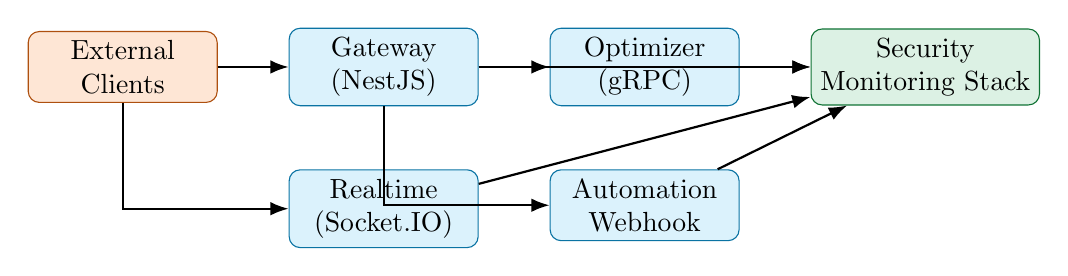
\begin{tikzpicture}[
  node distance=0.8cm and 0.9cm,
  box/.style={draw, rounded corners, align=center, minimum width=2.4cm, minimum height=0.9cm, fill=softgray},
  ext/.style={box, fill=accentorange!18, draw=accentorange!70!black},
  core/.style={box, fill=accentblue!15, draw=accentblue!70!black},
  sec/.style={box, fill=accentgreen!15, draw=accentgreen!70!black},
  arr/.style={-Latex, thick}
]
\node[ext] (clients) {External\\Clients};
\node[core, right=of clients] (gateway) {Gateway\\(NestJS)};
\node[core, below=of gateway] (realtime) {Realtime\\(Socket.IO)};
\node[core, right=of gateway] (optimizer) {Optimizer\\(gRPC)};
\node[core, below=of optimizer] (automation) {Automation\\Webhook};
\node[sec, right=of optimizer] (monitoring) {Security\\Monitoring Stack};

\draw[arr] (clients) -- (gateway);
\draw[arr] (clients) |- (realtime);
\draw[arr] (gateway) -- (optimizer);
\draw[arr] (gateway) |- (automation);
\draw[arr] (gateway) -- (monitoring);
\draw[arr] (realtime) -- (monitoring);
\draw[arr] (automation) -- (monitoring);
\draw[arr] (optimizer) -- (monitoring);
\end{tikzpicture}
\caption{High-level LogiFlow architecture and security-observable boundaries.}
\label{fig:architecture}
\end{figure}

\section{Threat Model}
Threats were scored using a simple operational risk equation:
\begin{equation}
R = L \times I
\end{equation}
where $L$ is likelihood (1--5) and $I$ is impact (1--5).

\begin{table}[htbp]
\caption{Highest-Priority Threats (Excerpt from STRIDE Register)}
\centering
\begin{tabularx}{\linewidth}{>{\raggedright\arraybackslash}p{1.2cm} X >{\centering\arraybackslash}p{1.1cm} >{\centering\arraybackslash}p{1.1cm} >{\centering\arraybackslash}p{1.2cm}}
\toprule
ID & Threat Scenario & L & I & Score \\
\midrule
TM-01 & Unauthorized subscription to vehicle socket rooms (Spoofing/Info Disclosure) & 5 & 5 & 25 \\
TM-02 & Forged webhook traffic events alter routing decisions (Spoofing/Tampering) & 4 & 5 & 20 \\
TM-03 & Webhook request flood creates service degradation (DoS) & 5 & 4 & 20 \\
TM-08 & Malicious process execution inside container runtime (EoP) & 4 & 5 & 20 \\
TM-11 & Exploitation of vulnerable dependencies in exposed service path & 4 & 4 & 16 \\
\bottomrule
\end{tabularx}
\label{tab:threats}
\end{table}

The mitigation order prioritized scores $\geq 20$ before medium-score controls, while preserving traceability to OWASP and NIST CSF.

\section{Unsecure vs Secure Architecture Comparison}
\begin{table*}[htbp]
\caption{Baseline Vulnerability to Implemented Security Control Mapping}
\centering
\begin{tabularx}{\textwidth}{>{\raggedright\arraybackslash}p{1.1cm} X X >{\raggedright\arraybackslash}p{2.6cm}}
\toprule
ID & Baseline Weakness & Implemented Control & Verification \\
\midrule
V-001 & Unauthenticated Socket.IO room subscription & JWT middleware enforced before join; unauthorized attempts counted as \texttt{logiflow\_socket\_unauthorized\_total} & Socket injection script returns authentication error \\
V-002 & Webhook endpoint accepts unauthenticated events & Bearer-protected webhook ingestion in gateway and automation flow & Unauthorized requests return HTTP 401 \\
V-003 & No rate limiting on traffic-event webhook & Request throttling and rate-limit counters/alerts & Flood scenarios produce HTTP 429 \\
V-005 & Missing hardening headers in gateway responses & Helmet + secure bootstrap configuration & Header verification by curl and DAST checks \\
V-006 & Verbose internal error exposure & Production-safe exception handling & Error responses sanitized under production profile \\
V-007 & Dependency exposure in service packages & CI SCA with \texttt{npm audit} policy and artifacts & Critical/high CVE counts monitored per service \\
V-008 & No runtime anomaly detection & Falco rules + Loki/Grafana runtime triage & Suspicious container behavior triggers alerts \\
\bottomrule
\end{tabularx}
\label{tab:beforeafter}
\end{table*}

The secure architecture also improved observability semantics by exposing metrics and traces from gateway and realtime services, reducing \emph{no data} states in dashboards and enabling direct triage links to tracing views.

\section{DevSecOps Pipeline Implementation}
\subsection{Pipeline Design}
The CI pipeline executes on push, pull request, schedule, and manual dispatch. It combines preventive and detective controls as shown in Fig.~\ref{fig:pipeline}.

\begin{figure}[htbp]
\centering
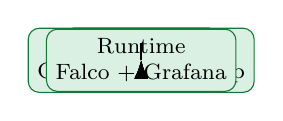
\begin{tikzpicture}[
  node distance=0.45cm and 0.45cm,
  stage/.style={draw, rounded corners, minimum width=2.0cm, minimum height=0.75cm, align=center, font=\footnotesize},
  left/.style={stage, fill=accentpurple!18, draw=accentpurple!80!black},
  right/.style={stage, fill=accentgreen!16, draw=accentgreen!75!black},
  sec/.style={stage, fill=accentorange!20, draw=accentorange!80!black},
  arr/.style={-Latex, thick}
]
\node[left] (code) {Code\\Commit};
\node[sec, right=of code] (sast) {SAST\\CodeQL + Semgrep};
\node[sec, right=of sast] (sca) {SCA\\npm audit};
\node[sec, right=of sca] (secrets) {Secrets\\GitLeaks};
\node[sec, right=of secrets] (trivy) {Container\\Trivy};
\node[sec, right=of trivy] (zap) {DAST\\OWASP ZAP};
\node[right, right=of zap] (runtime) {Runtime\\Falco + Grafana};

\draw[arr] (code) -- (sast);
\draw[arr] (sast) -- (sca);
\draw[arr] (sca) -- (secrets);
\draw[arr] (secrets) -- (trivy);
\draw[arr] (trivy) -- (zap);
\draw[arr] (zap) -- (runtime);
\end{tikzpicture}
\caption{Security pipeline from shift-left analysis to runtime monitoring.}
\label{fig:pipeline}
\end{figure}

\subsection{Implemented Gates and Hardening Details}
\begin{itemize}
\item \textbf{SAST}: CodeQL and Semgrep rulepacks for JavaScript/TypeScript analysis.
\item \textbf{SCA}: Per-service audit artifacts with criticality evaluation logic.
\item \textbf{Secrets}: GitLeaks baseline in all push/PR paths.
\item \textbf{Container Security}: Trivy config scan over gateway Docker context, including non-root requirement remediation.
\item \textbf{DAST}: OWASP ZAP baseline against gateway health target, with parser-based gating.
\item \textbf{CI Reliability Hardening}: automatic creation of \texttt{logiflow-security-net} in CI before DAST service startup.
\end{itemize}

\section{Continuous Monitoring and Triage Stack}
\subsection{Metrics, Logs, Runtime Alerts, and Traces}
The monitoring stack includes Falco, Prometheus, Loki, Grafana, Tempo, and OpenTelemetry Collector. Gateway and realtime services export security-oriented metrics and traces.

\begin{table}[htbp]
\caption{Representative Security Telemetry Signals}
\centering
\begin{tabularx}{\linewidth}{>{\raggedright\arraybackslash}p{2.9cm} >{\raggedright\arraybackslash}X}
\toprule
Signal & Security Meaning \\
\midrule
\texttt{logiflow\_auth\_failures\_total} & Failed authentication attempts in gateway \\
\texttt{logiflow\_webhook\_requests\_total} & Inbound webhook request activity \\
\texttt{logiflow\_socket\_unauthorized\_total} & Unauthorized socket connection attempts \\
\texttt{logiflow\_socket\_connections\{role\}} & Active real-time sessions by role \\
Falco critical alerts & Syscall-level runtime anomalies and policy violations \\
Tempo traces (OTel) & Cross-service execution and forensic timing correlation \\
\bottomrule
\end{tabularx}
\label{tab:telemetry}
\end{table}

\subsection{Dashboards and Navigation Improvements}
Three security dashboards were stabilized with no-data-safe queries and fast refresh windows. A dedicated traces dashboard was added, plus panel-level links from high-signal panels (Auth Failures and Falco Critical Alerts) directly to Grafana Explore with Tempo preselected. This reduced analyst friction during incident triage.

\section{Evaluation and Results}
\subsection{Test Plan Coverage}
The security test plan defines TC-01 to TC-10 spanning auth bypass, socket abuse, DoS, injection checks, header validation, secrets, dependencies, runtime anomalies, JWT tampering, and error disclosure.

\begin{table}[htbp]
\caption{Validation Summary for Core Security Scenarios}
\centering
\begin{tabularx}{\linewidth}{>{\raggedright\arraybackslash}p{1.1cm} X >{\centering\arraybackslash}p{1.1cm}}
\toprule
Test & Security Objective & Result \\
\midrule
TC-01 & Enforce authentication on protected endpoints & Pass \\
TC-02 & Reject unauthorized socket joins & Pass \\
TC-03 & Trigger rate-limit under flood conditions & Pass \\
TC-04/05 & Detect injection/header issues via DAST baseline & Pass (no blocking high findings in hardened target) \\
TC-06 & Prevent leaked credentials in repository & Pass \\
TC-07 & Track dependency vulnerabilities by service & Pass with policy-driven gating \\
TC-08 & Detect suspicious container behavior at runtime & Pass \\
TC-09 & Reject manipulated JWT privilege escalation & Pass \\
TC-10 & Avoid internal error leakage in production mode & Pass \\
\bottomrule
\end{tabularx}
\label{tab:results}
\end{table}

\subsection{Operational Outcomes}
Compared to the vulnerable baseline, the hardened architecture provides:
\begin{itemize}
\item Stronger prevention for external exploit paths (API, sockets, webhooks).
\item Earlier defect detection in CI through layered static and dynamic checks.
\item Better runtime detection and faster triage via correlated metrics, logs, and traces.
\end{itemize}

\section{SPTI Course Concepts Mapping}
\begin{table*}[htbp]
\caption{SPTI Concept-to-Artifact Traceability}
\centering
\begin{tabularx}{\textwidth}{>{\raggedright\arraybackslash}p{3.2cm} X >{\raggedright\arraybackslash}p{3.0cm}}
\toprule
SPTI Concept & Evidence in This Work & Practical Outcome \\
\midrule
Risk Management & STRIDE register with risk equation $R=L\times I$ and prioritization bands & Structured treatment order for highest-impact threats \\
Security Architecture Principles & JWT guards, bearer enforcement, rate limiting, exception hardening, least-privilege runtime & Reduced attack success probability at trust boundaries \\
SGSI / Governance & NIST-mapped controls matrix, CI evidence artifacts, repeatable test criteria & Auditability and traceable control ownership \\
Data Protection & Secrets detection, controlled token flows, reduced unauthorized telemetry exposure & Improved confidentiality and accountability \\
Software Security & CodeQL, Semgrep, Trivy, ZAP, dependency audit, runtime alerts & Continuous security quality gates and faster remediation \\
Continuous Monitoring & Falco + Prometheus + Loki + Grafana + Tempo + OTel collector & End-to-end incident detection and correlated investigation \\
\bottomrule
\end{tabularx}
\label{tab:spti}
\end{table*}

\section{Conclusions and Future Work}
This paper demonstrated a full DevSecOps monitoring architecture for LogiFlow that is reproducible, evidence-driven, and aligned with academic security objectives. The transition from a vulnerable baseline to a hardened architecture produced concrete benefits in preventive controls, runtime detection, and incident triage readiness.

Future work will focus on: (i) automated secret rotation and vault-backed credential governance, (ii) SOAR-style incident orchestration for Falco/Prometheus alerts, (iii) stronger policy-as-code baselines for supply-chain controls, and (iv) longitudinal quantitative benchmarking of mean time to detect and mean time to respond.

\section*{Acknowledgment}
This work was developed in the context of the SPTI course at Escuela Colombiana de Ingenieria Julio Garavito.

\bibliographystyle{IEEEtran}
\bibliography{references}

\end{document}
